\documentclass{ees}

\newgeometry{twoside=false,left=20mm,right=40mm,top=20mm,bottom=40mm}

\newlist{bulletlist}{itemize}{1}
\setlist[bulletlist]{
  partopsep=0pt,
  parsep=0pt,
  itemsep=0pt,
  label=\textbullet
}

\setcounter{tocdepth}{1}
\DeclareTOCStyleEntry[
  indent=0pt,
  beforeskip=\baselineskip,
  entrynumberformat=\@gobble,
  entryformat=\sbseries,
  numwidth=2em,
  linefill=\hfill,
  pagenumberbox=\pnumbox,
  pagenumberformat=\sbseries
]{tocline}{chapter}

\hyphenation{Mu-sik-ar-chiv}
\begin{document}

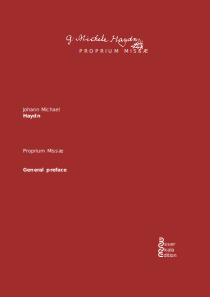
\includepdf{cover_general_preface.pdf}
\pagenumbering{arabic}
\setcounter{page}{1}

\tableofcontents

\chapter{General preface}

\textit{Johann Michael Haydn: Proprium Missæ} (JMH:PM) is an edition project that will make Haydn’s short liturgical works available in modern editions.


\section{Editorial guidelines}

In general, JMH:PM follows the \href{https://edition.esser-skala.at/about/editorial-guidelines/}{editorial guidelines} for the Edition Esser-Skala.


\section{Acknowledgements}

Assistance of the following people and institutions is gratefully acknowledged:
Thomas Dolezal (Dommusikarchiv Eisenstadt – A-Ed),
P. Roman Nägele (Stift Heiligenkreuz im Wienerwald, Musikarchiv – A-HE),
P. Altman Pötsch (Benediktinerstift Kremsmünster, Regenterei und Musikarchiv – A-KR),
Peter Deinhammer (Benediktinerstift Lambach, Musikarchiv – A-LA),
N.N. (Musikarchiv Stift Reichersberg – A-RB),
as well as the staff of
the Röm. Kath. Pfarramt Spitz an der Donau (A-SPD),
the Österreichische Nationalbibliothek, Musiksammlung, Wien (A-Wn),
the Wienbibliothek im Rathaus, Musiksammlung (A-Wst),
the Národní knihovna České republiky, Praha (CZ-Pu),
the Staatsbibliothek zu Berlin - Preußischer Kulturbesitz, Musikabteilung (D-B),
the Universitätsbibliothek Eichstätt-Ingolstadt (D-Eu),
the Bayerische Staatsbibliothek, München (D-Mbs),
the Benediktinerabtei Niederaltaich - St. Mauritius (D-NATk),
the Badische Landesbibliothek, Musiksammlung, Karlsruhe (D-KA),
the Bibliothèque nationale de France, Département de la Musique, Paris (F-Pn),
the British Library, London (GB-Lbl), and
the Library of Congress, Music Division, Washington, D.C. (US-Wc).


\clearpage
\markdownInput{../CHANGELOG.md}

\end{document}
